%% This file has been modified by igattr
%% Do not edit manually
%\VignetteIndexEntry{pbkrtest-introduction: Introduction to pbkrtest}
%\VignettePackage{pbkrtest}

\documentclass[11pt]{article}
\usepackage{url,a4}

\usepackage[latin1]{inputenc}
%\usepackage{inputenx}
\usepackage{boxedminipage,color}
\usepackage[noae]{Sweave}

\parindent0pt\parskip5pt
\def\code#1{{\texttt{#1}}}
\def\pkg#1{{\texttt{#1}}}
\def\R{\texttt{R}}





\title{On the usage of the  \pkg{pbkrtest} package}
\author{S{\o}ren H{\o}jsgaard and Ulrich Halekoh}
\date{\pkg{pbkrtest} version 0.4-1 as of 2014-09-09}



\begin{document}

\definecolor{darkred}{rgb}{.7,0,0}
\definecolor{midnightblue}{rgb}{0.098,0.098,0.439}

\DefineVerbatimEnvironment{Sinput}{Verbatim}{
  fontfamily=tt,
  %%fontseries=b,
  %% xleftmargin=2em,
  formatcom={\color{midnightblue}}
}
\DefineVerbatimEnvironment{Soutput}{Verbatim}{
  fontfamily=tt,
  %%fontseries=b,
  %% xleftmargin=2em,
  formatcom={\color{darkred}}
}
\DefineVerbatimEnvironment{Scode}{Verbatim}{
  fontfamily=tt,
  %%fontseries=b,
  %% xleftmargin=2em,
  formatcom={\color{blue}}
}

\fvset{listparameters={\setlength{\topsep}{-2pt}}}
\renewenvironment{Schunk}{\linespread{.90}}{}



\maketitle
\tableofcontents


%% useFancyQuotes = FALSE

\section{Introduction}

The \code{shoes} data is a list of two vectors, giving the wear of
shoes of materials A and B for one foot each of ten boys.

\begin{Schunk}
\begin{Sinput}
R> data(shoes, package="MASS")
R> shoes
\end{Sinput}
\begin{Soutput}
$A
 [1] 13.2  8.2 10.9 14.3 10.7  6.6  9.5 10.8  8.8 13.3

$B
 [1] 14.0  8.8 11.2 14.2 11.8  6.4  9.8 11.3  9.3 13.6
\end{Soutput}
\end{Schunk}

A plot clearly reveals that boys wear their shoes differently.

\begin{Schunk}
\begin{Sinput}
R> plot(A~1, data=shoes, col="red",lwd=2, pch=1, ylab="wear", xlab="boy")
R> points(B~1, data=shoes, col="blue", lwd=2, pch=2)
R> points(I((A+B)/2)~1, data=shoes, pch="-", lwd=2)
\end{Sinput}
\end{Schunk}
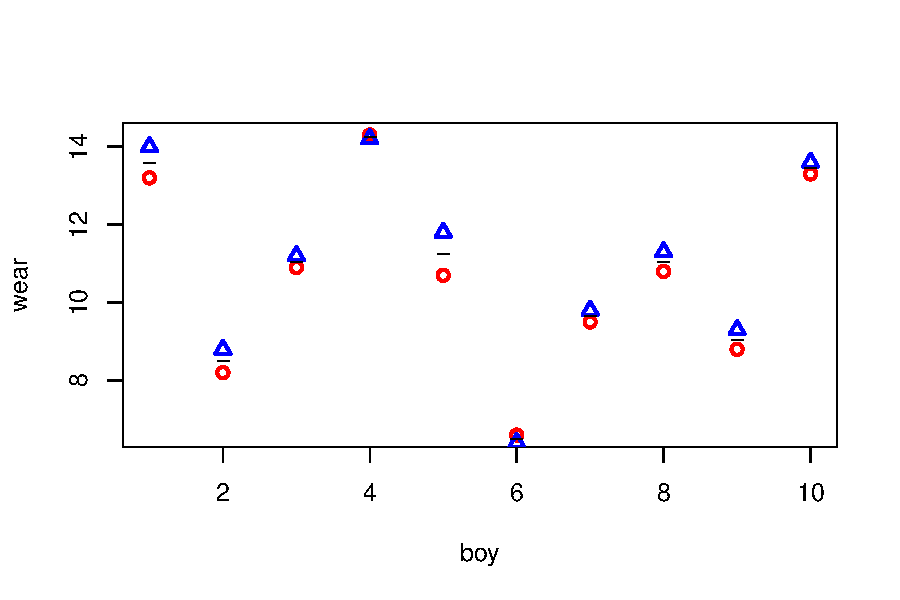
\includegraphics{figures/pbkr-005}


One option for testing the effect of materials is to make a paired
$t$--test. The following forms are equivalent:

\begin{Schunk}
\begin{Sinput}
R> r1<-t.test(shoes$A, shoes$B, paired=T)
R> r2<-t.test(shoes$A-shoes$B)
R> r1
\end{Sinput}
\begin{Soutput}
	Paired t-test

data:  shoes$A and shoes$B
t = -3.3489, df = 9, p-value = 0.008539
alternative hypothesis: true difference in means is not equal to 0
95 percent confidence interval:
 -0.6869539 -0.1330461
sample estimates:
mean of the differences 
                  -0.41 
\end{Soutput}
\end{Schunk}


To work with data in a mixed model setting we create a dataframe, and
for later use we also create an imbalanced version of data:

\begin{Schunk}
\begin{Sinput}
R> boy <- rep(1:10,2)
R> boyf<- factor(letters[boy])
R> mat <- factor(c(rep("A", 10), rep("B",10)))
R> ## Balanced data:
R> shoe.b <- data.frame(wear=unlist(shoes), boy=boy, boyf=boyf, mat=mat)
R> head(shoe.b)
\end{Sinput}
\begin{Soutput}
   wear boy boyf mat
A1 13.2   1    a   A
A2  8.2   2    b   A
A3 10.9   3    c   A
A4 14.3   4    d   A
A5 10.7   5    e   A
A6  6.6   6    f   A
\end{Soutput}
\begin{Sinput}
R> ## Imbalanced data; delete (boy=1, mat=1) and (boy=2, mat=b)
R> shoe.i <-  shoe.b[-c(1,12),]
\end{Sinput}
\end{Schunk}

We fit models to the two datasets:

\begin{Schunk}
\begin{Sinput}
R> lmm1.b  <- lmer( wear ~ mat + (1|boyf), data=shoe.b )
R> lmm0.b  <- update( lmm1.b, .~. - mat)
R> lmm1.i  <- lmer( wear ~ mat + (1|boyf), data=shoe.i )
R> lmm0.i  <- update(lmm1.i, .~. - mat)
\end{Sinput}
\end{Schunk}

The asymptotic likelihood ratio test shows stronger significance than
the $t$--test:

\begin{Schunk}
\begin{Sinput}
R> anova( lmm1.b, lmm0.b, test="Chisq" ) ## Balanced data
\end{Sinput}
\begin{Soutput}
Data: shoe.b
Models:
lmm0.b: wear ~ (1 | boyf)
lmm1.b: wear ~ mat + (1 | boyf)
       Df    AIC    BIC  logLik deviance Chisq Chi Df Pr(>Chisq)   
lmm0.b  3 67.909 70.896 -30.955   61.909                           
lmm1.b  4 61.817 65.800 -26.909   53.817 8.092      1   0.004446 **
---
Signif. codes:  0 '***' 0.001 '**' 0.01 '*' 0.05 '.' 0.1 ' ' 1
\end{Soutput}
\begin{Sinput}
R> anova( lmm1.i, lmm0.i, test="Chisq" ) ## Imbalanced data
\end{Sinput}
\begin{Soutput}
Data: shoe.i
Models:
lmm0.i: wear ~ (1 | boyf)
lmm1.i: wear ~ mat + (1 | boyf)
       Df    AIC    BIC  logLik deviance Chisq Chi Df Pr(>Chisq)  
lmm0.i  3 63.869 66.540 -28.934   57.869                          
lmm1.i  4 60.777 64.339 -26.389   52.777 5.092      1    0.02404 *
---
Signif. codes:  0 '***' 0.001 '**' 0.01 '*' 0.05 '.' 0.1 ' ' 1
\end{Soutput}
\end{Schunk}

\section{Kenward--Roger approach}
\label{sec:kenw-roger-appr}


The Kenward--Roger approximation is exact for the balanced data in the
sense that it produces the same result as the paired $t$--test.

\begin{Schunk}
\begin{Sinput}
R> ( kr.b<-KRmodcomp(lmm1.b, lmm0.b) )
\end{Sinput}
\begin{Soutput}
F-test with Kenward-Roger approximation; computing time: 0.08 sec.
large : wear ~ mat + (1 | boyf)
small : wear ~ (1 | boyf)
        stat    ndf    ddf F.scaling  p.value   
Ftest 11.215  1.000  9.000         1 0.008539 **
---
Signif. codes:  0 '***' 0.001 '**' 0.01 '*' 0.05 '.' 0.1 ' ' 1
\end{Soutput}
\end{Schunk}

\begin{Schunk}
\begin{Sinput}
R> summary( kr.b )
\end{Sinput}
\begin{Soutput}
F-test with Kenward-Roger approximation; computing time: 0.08 sec.
large : wear ~ mat + (1 | boyf)
small : wear ~ (1 | boyf)
         stat    ndf    ddf F.scaling  p.value   
Ftest  11.215  1.000  9.000         1 0.008539 **
FtestU 11.215  1.000  9.000           0.008539 **
---
Signif. codes:  0 '***' 0.001 '**' 0.01 '*' 0.05 '.' 0.1 ' ' 1
\end{Soutput}
\end{Schunk}

Relevant information can be retrieved with

\begin{Schunk}
\begin{Sinput}
R> getKR(kr.b, "ddf")
\end{Sinput}
\begin{Soutput}
[1] 9
\end{Soutput}
\end{Schunk}

For the imbalanced data we get
\begin{Schunk}
\begin{Sinput}
R> ( kr.i<-KRmodcomp(lmm1.i, lmm0.i) )
\end{Sinput}
\begin{Soutput}
F-test with Kenward-Roger approximation; computing time: 0.08 sec.
large : wear ~ mat + (1 | boyf)
small : wear ~ (1 | boyf)
        stat    ndf    ddf F.scaling p.value  
Ftest 5.9893 1.0000 7.0219         1 0.04418 *
---
Signif. codes:  0 '***' 0.001 '**' 0.01 '*' 0.05 '.' 0.1 ' ' 1
\end{Soutput}
\end{Schunk}

Notice that this result is similar to but not identical to the paired
$t$--test when the two relevant boys are removed:

\begin{Schunk}
\begin{Sinput}
R> shoes2 <- list(A=shoes$A[-(1:2)], B=shoes$B[-(1:2)])
R> t.test(shoes2$A, shoes2$B, paired=T)
\end{Sinput}
\begin{Soutput}
	Paired t-test

data:  shoes2$A and shoes2$B
t = -2.3878, df = 7, p-value = 0.04832
alternative hypothesis: true difference in means is not equal to 0
95 percent confidence interval:
 -0.671721705 -0.003278295
sample estimates:
mean of the differences 
                -0.3375 
\end{Soutput}
\end{Schunk}


\section{Parametric bootstrap}
\label{sec:parametric-bootstrap}

Parametric bootstrap provides an alternative but many simulations are
often needed to provide credible results (also many more than shown
here; in this connection it can be useful to exploit that computings
can be made en parallel, see the documentation):

\begin{Schunk}
\begin{Sinput}
R> ( pb.b <- PBmodcomp(lmm1.b, lmm0.b, nsim=500) )
\end{Sinput}
\begin{Soutput}
Parametric bootstrap test; time: 14.07 sec; samples: 500 extremes: 1;
large : wear ~ mat + (1 | boyf)
small : wear ~ (1 | boyf)
         stat df  p.value   
LRT    8.1197  1 0.004379 **
PBtest 8.1197    0.003992 **
---
Signif. codes:  0 '***' 0.001 '**' 0.01 '*' 0.05 '.' 0.1 ' ' 1
\end{Soutput}
\end{Schunk}

\begin{Schunk}
\begin{Sinput}
R> summary( pb.b )
\end{Sinput}
\begin{Soutput}
Parametric bootstrap test; time: 14.07 sec; samples: 500 extremes: 1;
large : wear ~ mat + (1 | boyf)
small : wear ~ (1 | boyf)
           stat     df    ddf  p.value   
PBtest   8.1197               0.003992 **
Gamma    8.1197               0.006571 **
Bartlett 7.3783 1.0000        0.006602 **
F        8.1197 1.0000 21.903 0.009348 **
LRT      8.1197 1.0000        0.004379 **
---
Signif. codes:  0 '***' 0.001 '**' 0.01 '*' 0.05 '.' 0.1 ' ' 1
\end{Soutput}
\end{Schunk}


For the imbalanced data, the result is similar to the result from the
paired $t$ test.

\begin{Schunk}
\begin{Sinput}
R> ( pb.i<-PBmodcomp(lmm1.i, lmm0.i, nsim=500) )
\end{Sinput}
\begin{Soutput}
Parametric bootstrap test; time: 13.72 sec; samples: 500 extremes: 28;
large : wear ~ mat + (1 | boyf)
small : wear ~ (1 | boyf)
         stat df p.value  
LRT    5.1151  1 0.02372 *
PBtest 5.1151    0.05788 .
---
Signif. codes:  0 '***' 0.001 '**' 0.01 '*' 0.05 '.' 0.1 ' ' 1
\end{Soutput}
\end{Schunk}

\begin{Schunk}
\begin{Sinput}
R> summary( pb.i )
\end{Sinput}
\begin{Soutput}
Parametric bootstrap test; time: 13.72 sec; samples: 500 extremes: 28;
large : wear ~ mat + (1 | boyf)
small : wear ~ (1 | boyf)
           stat     df    ddf p.value  
PBtest   5.1151               0.05788 .
Gamma    5.1151               0.05270 .
Bartlett 3.8545 1.0000        0.04961 *
F        5.1151 1.0000 8.1155 0.05313 .
LRT      5.1151 1.0000        0.02372 *
---
Signif. codes:  0 '***' 0.001 '**' 0.01 '*' 0.05 '.' 0.1 ' ' 1
\end{Soutput}
\end{Schunk}


\appendix

\section{Matrices for random effects}
\label{sec:matr-rand-effects}

The matrices involved in the random effects can be obtained with

\begin{Schunk}
\begin{Sinput}
R> shoe3 <- subset(shoe.b, boy<=5)
R> shoe3 <- shoe3[order(shoe3$boy), ]
R> lmm1  <- lmer( wear ~ mat + (1|boyf), data=shoe3 )
R> str( SG <- get_SigmaG( lmm1 ), max=2)
\end{Sinput}
\begin{Soutput}
List of 3
 $ Sigma   :Formal class 'dgCMatrix' [package "Matrix"] with 6 slots
 $ G       :List of 2
  ..$ :Formal class 'dgCMatrix' [package "Matrix"] with 6 slots
  ..$ :Formal class 'dgCMatrix' [package "Matrix"] with 6 slots
 $ n.ggamma: int 2
\end{Soutput}
\end{Schunk}

\begin{Schunk}
\begin{Sinput}
R> round( SG$Sigma*10 )
\end{Sinput}
\begin{Soutput}
10 x 10 sparse Matrix of class "dgCMatrix"
                                   
 [1,] 53 52  .  .  .  .  .  .  .  .
 [2,] 52 53  .  .  .  .  .  .  .  .
 [3,]  .  . 53 52  .  .  .  .  .  .
 [4,]  .  . 52 53  .  .  .  .  .  .
 [5,]  .  .  .  . 53 52  .  .  .  .
 [6,]  .  .  .  . 52 53  .  .  .  .
 [7,]  .  .  .  .  .  . 53 52  .  .
 [8,]  .  .  .  .  .  . 52 53  .  .
 [9,]  .  .  .  .  .  .  .  . 53 52
[10,]  .  .  .  .  .  .  .  . 52 53
\end{Soutput}
\end{Schunk}

\begin{Schunk}
\begin{Sinput}
R> SG$G
\end{Sinput}
\begin{Soutput}
[[1]]
10 x 10 sparse Matrix of class "dgCMatrix"
                         
 [1,] 1 1 . . . . . . . .
 [2,] 1 1 . . . . . . . .
 [3,] . . 1 1 . . . . . .
 [4,] . . 1 1 . . . . . .
 [5,] . . . . 1 1 . . . .
 [6,] . . . . 1 1 . . . .
 [7,] . . . . . . 1 1 . .
 [8,] . . . . . . 1 1 . .
 [9,] . . . . . . . . 1 1
[10,] . . . . . . . . 1 1

[[2]]
10 x 10 sparse Matrix of class "dgCMatrix"
                         
 [1,] 1 . . . . . . . . .
 [2,] . 1 . . . . . . . .
 [3,] . . 1 . . . . . . .
 [4,] . . . 1 . . . . . .
 [5,] . . . . 1 . . . . .
 [6,] . . . . . 1 . . . .
 [7,] . . . . . . 1 . . .
 [8,] . . . . . . . 1 . .
 [9,] . . . . . . . . 1 .
[10,] . . . . . . . . . 1
\end{Soutput}
\end{Schunk}




\end{document}



% \section{With linear models}
% \label{sec:with-linear-models}


% @
% <<>>=
% lm1.b <- lm( wear ~ mat + boyf, data=shoe.b )
% lm0.b <- update( lm1.b, .~. - mat )
% anova( lm1.b, lm0.b )
% @ %def


% @
% <<>>=
% lm1.i <- lm( wear ~ mat + boyf, data=shoedf2 )
% lm0.i <- update( lm1.i, .~. - mat )
% anova( lm1.i, lm0.i )
% @ %def

